\chapter{COFFEE: a Compiler for Fast Expression Evaluation}
\label{ch:coffee}

Sharing elimination and pre-evaluation, presented in Chapter~\ref{ch:optimality}, as well as the low level optimizations in Chapter~\ref{ch:lowlevelopt}, have been implemented in COFFEE\footnote{COFFEE is the acronym for COmpiler For Fast Expression Evaluation.}, a high-level compiler integrated with Firedrake. In this chapter, the conception, architecture and interface of COFFEE are described. The codebase, which comprises more than 4000 lines of Python, is available at~\citep{coffee-code}.


\section{Overview}

We recall from Section~\ref{sec:bkg:fenics-and-firedrake} that Firedrake users employ the Unified Form Language to express problems in a mathematical syntax. At run-time, the high-level specification is translated by a form compiler, the Two-Stage Form Compiler (TSFC)~\citep{TSFC}, into one or more abstract syntax trees (ASTs) representing assembly kernels\footnote{TSFC has recently replaced FFC, the FEniCS Form Compiler, which has been used for performance evaluation in the previous chapters.}. ASTs are then passed to COFFEE for optimization. The output of COFFEE, C code, is eventually provided to PyOP2~\citep{pyop2isc}, where just-in-time compilation and execution over the computational mesh take place. This structure of this tool-chain is outlined in Figure~\ref{fig:coffee-pipeline}, along with an overview of the compilation pipeline in COFFEE. 

\begin{figure}
\centering
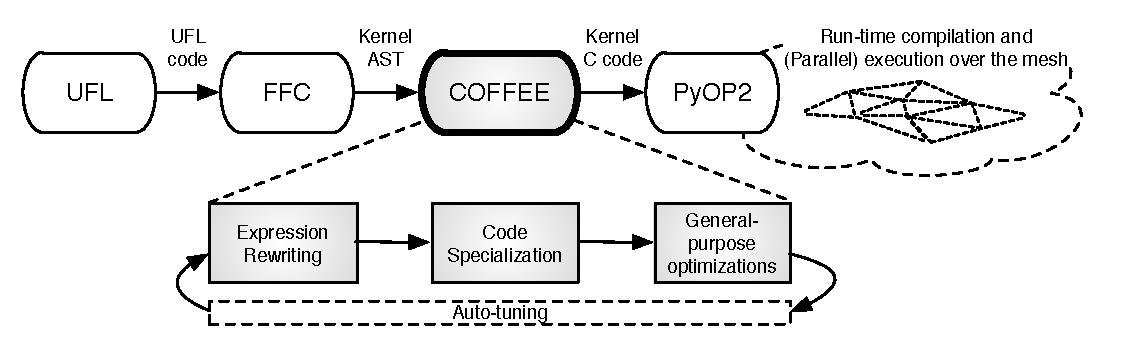
\includegraphics[scale=0.50]{coffee/pictures/coffee-pipeline.pdf}
\caption{The COFFEE's compilation pipeline and its interaction with Firedrake.}
\label{fig:coffee-pipeline}
\end{figure}

\section{The Compilation Pipeline}
\label{sec:coffee:pipeline}
In common with general-purpose compilers, COFFEE provides multiple optimization levels: \texttt{O0}, \texttt{O1}, \texttt{O2} and \texttt{O3}. Apart from \texttt{O0}, which essentially leaves the ASTs unchanged (useful for debugging), all optimization levels apply ordered sequences of transformations. In essence, the higher the optimization level, the more aggressive (and potentially slower) is the AST processing. In the following, when describing aspects of the optimization process common to \texttt{O1}, \texttt{O2} and \texttt{O3}, we will use the generic notation \texttt{Ox} (\texttt{x} $\in \lbrace 1, 2, 3\rbrace$).

The optimization level \texttt{Ox} can logically be split into three stages:
\begin{description}
\item[Expression rewriting] Any transformations changing the structure of an expression. These are sharing elimination and pre-evaluation; or, more in general, any rewrite operators on top of which such higher level transformations are expressed (e.g., generalized code motion, factorization; full list provided in Section~\ref{sec:coffee:rewrite-ops}). 
\item[Sparsity Optimization] The iteration spaces are restructured to skip useless operations, such as those involving blocks of zeros in basis function tables. In particular, loops may be fissioned, their bounds changed, and offsets introduced for accessing non-zero array values. More details are presented in Section~\ref{sec:zeros}.
\item[Code Specialization] A combination of the low level transformations presented in Chapter~\ref{ch:coffee} is applied.
\end{description}
These three stages are totally ordered. Indeed, it would be useless to apply any of the low level transformations until all loops and temporaries have been created.

The optimization process \texttt{Ox} represents the core phase in COFFEE. Overall, the compilation pipeline consists of three phases:

\begin{description}
\item[Analysis] During the analysis phase, an AST is visited and information are collected. In particular, candidates for expression rewriting are searched for. These are represented as special nodes in the AST, which we refer to as ``expression nodes''. In plain C, we could think of an expression node as a statement preceded by a directive such as \texttt{$\#$pragma coffee}. The purpose of the directive would be to trigger COFFEE's \texttt{Ox}, similarly to the way loops are parallelized through OpenMP. If no expression nodes are found, we jump directly to the last phase (i.e., code generation).

\item[Optimization ({\tt Ox} or user-provided)] In addition to \texttt{Ox}, users can craft their own optimization pipelines by composing the individual transformations available in COFFEE. The compiler checks that the provided transformation sequence is legal. If the specified sequence of transformations is legal, the AST is processed. Specifically, for {\tt Ox}:
\begin{description}
\item[\texttt{O1}] Expression rewriting reduces to generalized code motion, while only padding and data alignment as well as loop fusion are applied amongst the low level optimizations.
\item[\texttt{O2}] With respect to \texttt{O1}, there is only one yet fundamental change: expression rewriting now performs the whole sharing elimination procedure (i.e., Algorithm~\ref{algo:sharing-elimination}).
\item[\texttt{O3}] Algorithm~\ref{algo:gamma}, which coordinates sharing elimination and pre-evaluation, is executed. This is followed by sparsity optimization, loop fusion and padding and data alignment.
\end{description}

\item[Code generation]
All optimizations have been applied, so a string representation of the transformed AST is produced and returned.
\end{description}

\section{Plugging COFFEE into Firedrake}
\label{sec:coffee-implementation}

In this section, we explain how COFFEE interacts with the Firedrake ecosystem.

\subsection{Abstract Syntax Trees}
We start with highlighting peculiarities of the hierarchy of AST nodes.

\paragraph{Special nodes}
Some nodes have special semantics. A first example is the {\it expression node} described in the previous section. Furthermore, a whole sub-hierarchy of \texttt{LinAlg} nodes is available, with objects such as \texttt{Invert} and \texttt{Determinant} representing basic linear algebra operation. Code generation for these objects can be specialized based upon the underlying architecture and the size of the involved tensors. For instance, a manually-optimized loop nest may be preferred to a BLAS function when the tensors are small\footnote{It is well-known that BLAS libraries are highly optimized for big tensors, while their performance tends to be sub-optimal with small tensors, which are very common in assembly kernels.}. Yet another special type of node is \texttt{ArrayInit}, used for static initialization of arrays. An \texttt{ArrayInit} wraps an $N$-dimensional Numpy array~\citep{Numpy} and provides a simple interface to obtain information useful for sparsity optimization, like the sparsity pattern of the array. 

\paragraph{Symbols}
A \texttt{Symbol} represents a variable in the code. The \textit{rank} of a \texttt{Symbol} captures the dimensionality of a variable, with a rank equal to $N$ indicating that the variable is an $N$-dimensional array ($N=0$ implies that the variable is a scalar). The rank is implemented as an $N$-tuple, each entry being either an integer or a string representing a loop dimension. The \textit{offset} of a \texttt{Symbol} is again an $N$-tuple where each element is a 2-tuple. For each entry $r$ in the rank, there is a corresponding entry ${<}scale,\ stride{>}$ in the offset. Rank and offset are used as in Figure~\ref{fig:coffee-ast-vs-c} to access specific memory locations. By clearly separating the rank and the offset of a \texttt{Symbol} -- rather than storing a generic expression -- the data dependency analysis required by the rewrite operators is greatly simplified. The underlying assumption is that all symbols' access functions (Section~\ref{sec:bkg:terminology}) are affine in the loop indices. This is definitely the case for the class of kernels in which we are interested.

\begin{figure}
\begin{center}
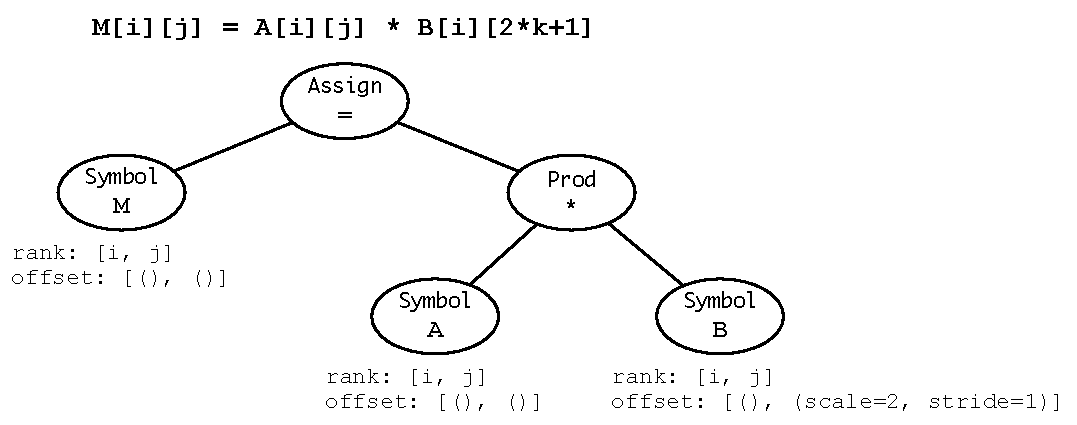
\includegraphics[scale=0.70]{coffee/pictures/coffee-ast.pdf}
\caption{AST representation of a C assignment in COFFEE.}
\label{fig:coffee-ast-vs-c}
\end{center}
\end{figure}

\paragraph{Building an AST}
Rather than using a parser, COFFEE exposes the whole hierarchy of nodes for explicitly building ASTs. This is because the compiler is meant to be used as an intermediate representation in a multilayer framework based on DSLs. To ease the construction of ASTs (especially nested loops), a set of utility functions is provided. 

\subsection{Integration with Form Compilers}
COFFEE has been integrated with two form compilers: the FEniCS Form Compiler (FFC) and the Two-Stage Form Compiler (TSFC). These form compilers represent assembly kernels using their own internal language. The objective is to turn such a representation into an AST suitable for COFFEE. 

\paragraph{FFC and COFFEE}
FFC was developed in the context of the FEniCS framework. We had to modify the FFC's intermediate representation for constructing COFFEE ASTs, rather than C code. We made the following changes:
\begin{itemize}
\item The mathematical expression evaluating the element tensor is represented in FFC as a tree data structure, or FFC AST. A limitation of an FFC AST was that its nodes -- symbols or arithmetic operations -- were not bound to loops. For instance, the FFC AST node corresponding to the symbol \texttt{A[i][j]} could not separate the variable name \texttt{A} from the loop indices \texttt{i} and \texttt{j}. We have enriched FFC AST symbols with additional fields to capture this kind of information.
\item Basis functions in an FFC AST are added a new field storing the dimensionality of the function space. This information is later used to enrich \texttt{ArrayInit} objects with a sparsity pattern. This enables sparsity optimization without requiring COFFEE to ``sniff'' array values.
\end{itemize}

The enriched FFC AST is intercepted prior to code generation and forwarded to a new module, where a COFFEE AST is constructed. In this module:
\begin{itemize}
\item the strings in the template originally used by FFC for code generation are now COFFEE AST objects.
\item the FFC AST is visited and translated into a COFFEE AST by a suitable AST-to-AST converter routine.
\end{itemize}

\paragraph{TSFC and COFFEE}
TSFC was conceived to produce an input suitable for COFFEE. This is accomplished through an AST-to-AST converter, which translates the GEM representation (the internal language used by TSFC) of an assembly kernel into a COFFEE AST. The implementation was carried out by Myklós Homolya, the lead designer of TSFC.


\section{Rewrite Operators}
\label{sec:coffee:rewrite-ops}
COFFEE implements sharing elimination and pre-evaluation by composing ``building-block'' operators, or ``rewrite operators''. This has several advantages. Firstly, extensibility: novel transformations -- for instance, sum-factorization in spectral methods -- could be expressed using the existing operators, or with small effort building on what is already available. Secondly, generality: COFFEE can be seen as a lightweight, low level computer algebra system, not necessarily tied to finite element integration. Thirdly, robustness: the same operators are exploited, and therefore stressed, by different optimization pipelines. The rewrite operators, whose implementation is based on manipulation of the kernel's AST, essentially compose the COFFEE language. 

The most important rewrite operators in COFFEE are:
\begin{description}
\item[Generalized code motion] A sub-expression that is invariant with respect to one or more loops can be hoisted at the level of an outer loop, thus reducing the operation count. This requires introducing a temporary (scalar, array) for each invariant sub-expression and, possibly, adding a ``clone'' loop to the nest (Several examples, e.g. Figure~\ref{code:loopnest}, have been provided throughout the thesis). 
\item[Expansion] Exploiting distributivity, this transformation expands a product between two sub-expressions. Expansion has several effects: (i) exposing factorization opportunities (see Chapter~\ref{ch:optimality}); (ii) increasing the operation count; (iii) in some circumstances, relieving the register pressure by creating code motion opportunities.
\item[Factorization] The impact of factorizing, or collecting, identical symbols is twofold: (i) reducing the number of multiplications to be performed; (ii) more importantly, exposing code motion opportunities, as illustrated through sharing elimination and pre-evaluation.
\item[Symbolic evaluation] This operator evaluates sub-expressions that only involve statically initialized, read-only arrays (e.g., basis function tables). The result is stored into a new array, and the AST modified accordingly
\end{description}
All these operators are used by both sharing elimination and pre-evaluation (apart from symbolic evaluation, only employed by pre-evaluation).

The rewrite operators accept a number of options to enable users to steer the transformation process. With code motion, for example, one can specify what kind of sub-expressions should be hoisted (by indicating the invariant loops) or the maximum amount of memory that is spendable in temporaries. Factorization can be either ``explicit'' -- in which case, a list of symbols to be collected or a loop dimension along which searching for factorizable symbols are provided -- or ``heuristic'' -- with groups of recurring identical symbols being collected.

\section{Features of the Implementation}
This section focuses on the toolkit available in COFFEE for implementing and extending rewrite operators.

\subsection{Tree Visitor Pattern}
The need for a generic infrastructure for traversing ASTs has grown rapidly, together with the complexity of the compiler. In the early stages of COFFEE, any time a new transformation (e.g., a rewrite operator) or inspector (e.g., for dependence analysis) was required, one or more full AST traversals had to be implemented. The lack of a common interface for tree traversals also made the code less homogeneous and, as such, more difficult to understand. This led to the introduction of a tree visitor design pattern\footnote{The tree visitor infrastructure was mainly developed by Lawrence Mitchell, and was inspired by that adopted in UFL, the language used to specify forms in Firedrake.}, whose aim is to decouple the algorithms from the data structure on which they are applied. 

As an example, consider an algorithm that needs to perform special actions when a \texttt{Symbol} or a \texttt{ForLoop} nodes are encountered (e.g., to collect loop dependence information). Then, a tree visitor will only need to implement three methods, namely \texttt{visit$\_$Symbol} and \texttt{visit$\_$ForLoop} -- the actual handlers -- as well as \texttt{visit$\_$Node}, which will implement the ``fallback'' action for all other node types (e.g., a propagation of the visit).

Tree visitors exploit the hierarchy of AST nodes by always dispatching to the most specialized handler. For example, symbols are simultaneously of type \texttt{Symbol} and \texttt{Expression}, but if a \texttt{Symbol} is encountered and \texttt{visit$\_$Symbol} is implemented, then \texttt{visit$\_$Symbol} is executed, whereas \texttt{visit$\_$Expression} (if any) is ignored.

Most of the algorithms in COFFEE exploit the tree visitor pattern.

\subsection{Flexible Code Motion}
\label{sec:coffee:cm}
Code motion consists of hoisting a sub-expression out of one or more loops. We already know that this operator is used in different contexts: as a stand-alone transformation (optimization level \texttt{O1}), to implement sharing elimination, and to implement pre-evaluation. 

When applying the operator, several pieces of information must be known:
\begin{itemize}
\item Which sub-expressions should be hoisted; for instance, should they be constant or invariant in at most one of the linear loops.
\item Where sub-expressions should be hoisted; that is, how far in the loop nest (which affects the size of the temporaries).
\item How much memory are we allowed to use in total for the temporaries.
\item A list of previously hoisted sub-expressions, for applying common sub-expressions elimination.
\end{itemize}

COFFEE tracks all of the hoisted sub-expressions for quick retrieval. A dictionary mapping temporaries to metadata is employed. For a temporary \texttt{t}, the dictionary records:
\begin{itemize}
\item A reference to the hoisted expression \texttt{e} assigned to \texttt{t}.
\item A reference to the loop in which \texttt{e} is lifted (if any).
\item A reference to the declaration of \texttt{t}.
\item Some extra fields.
\end{itemize}
This dictionary is updated after each invocation to the code motion operator and forms part of the ``global state'' that COFFEE maintains for each assembly kernel. Not only is the dictionary accessed by later calls to the code motion operator, but also by other operators, thus speeding-up the AST transformation process.

The code motion operator ``silently'' applies common sub-expressions elimination. A look-up to the dictionary tells whether a hoistable sub-expression \texttt{e} has already been assigned to a temporary \texttt{t} by a prior call to the operator; in such a case, \texttt{e} is replaced with \texttt{t} and no useless temporaries are introduced. 

%The code motion operator is ``smart'', in the sense that common sub-expressions,  every time a sub-expression is about to be hoisted, \texttt{e} is lifted out of the iteration space \texttt{I}, three further ``extra'' optimizations are attempted. 
%
%\begin{description}
%\item[Identification of common sub-expression] If a semantically equivalent sub-expression \texttt{e'} had been hoisted along the same iteration space \texttt{I}, then \texttt{e} is rather replaced with a reference to the temporary that \texttt{e'} is assigned to.
%\item[Loop fusion.] When test and trial functions belong to the same function space, common sub-expressions may arise over different loops.  


\subsection{Tracking Data Dependency}
Data dependency analysis is necessary to ensure the legality of transformations. For example:
\begin{itemize}
\item We may want to hoist a sub-expression \texttt{e} ``as far as possible'' in the loop nest, but after the last write to a variable read in \texttt{e}.
\item When expanding a product, some terms may be aggregated with previously hoisted sub-expressions. This would avoid introducing extra temporaries and increasing the register pressure. For example, if we have \texttt{(a + b)*c} and both \texttt{a} and \texttt{b} are temporaries created by code motion, we could expand the product and aggregate \texttt{c} with the sub-expressions stored by \texttt{a} and \texttt{b}. Obviously, this is legal as long as neither \texttt{a} nor \texttt{b} are accessed in other sub-expressions.
\item To check whether fusing a sequence of loops is legal (see Section~\ref{sec:coffee-loopfusion}).
\item To implement the {\em strategy selection analysis} in Section~\ref{sec:opt:driving-se}.
\end{itemize}

COFFEE uses a dependency graph to track data dependencies. The dependency graph has as many vertices as symbols in the code; a direct edge from \texttt{A} to \texttt{B} indicates that symbol \texttt{B} depends on (i.e., is going to read) symbol \texttt{A}. Since COFFEE relies on \textit{static single assignment} -- a property that ensures that variables are assigned exactly once -- such a minimalistic data structure suffices for data dependence analysis.

\subsection{Minimizing Temporaries}
Both the code motion operator and loop fusion (Section~\ref{sec:coffee-loopfusion}) impact the number of temporaries in an assembly kernel. Once the AST has been transformed, a special routine attempts to remove the unnecessary temporaries. In addition to relieving the register pressure (this actually depends on how smart the underlying general-purpose compiler is), this has the effect of making the code more readable.

The main rule for removing a temporary \texttt{t} storing an expression \texttt{e} is that if \texttt{t} is accessed only in a single statement \texttt{s}, then \texttt{e} is inlined into \texttt{s} and \texttt{t} is removed. Secondly, if some of the transformations in the optimization pipeline reduced \texttt{e} to a symbol, then any appearance of \texttt{t} is also replaced by \texttt{e}.

\section{On the Compilation Time}
Firedrake and its various software components are implemented in Python, whereas the generated code is pure C. COFFEE has been written in Python for a natural integration with Firedrake. The process of transforming an AST usually takes fractions of seconds. For more complex forms, on a Sandy Bridge architecture, the AST processing takes not more than approximately 2 seconds. For extremely challenging forms, like those arising in the Holzapfel-Ogden hyperelasticity model, the code generation is carried out in 16 seconds; this is the only case, out of dozens, in which the processing time was higher than 3 seconds. We believe, however, that there is still ample space for optimizing the AST processing in COFFEE.
